\documentclass[10pt]{article}

\usepackage[utf8]{inputenc}
\usepackage{lmodern}
\usepackage{amsmath}
\usepackage{graphicx}
\usepackage{microtype}

\setlength{\columnsep}{0.85cm}  % Adjust spacing between columns if desired

\begin{document}

\twocolumn[
\begin{center}
\LARGE \textbf{Information Retrieval and Data Mining (COMP0084) Coursework 1} \\
\vspace{0.5em}
\end{center}
]

\noindent
\section*{Abstract:} This coursework looks into developing an information retrieval model that generates a ranked list of passages relevant to a given query and ensures that the most relevant passages are at the top. There are four parts within this coursework which are: Task 1 - create a function to process raw text and compare empirical term distribution with Zipf’s law, Task 2 – develop an inverted index to facilitate more efficient passage retrieval, Task 3 – Implement TF-IDF and BM25 retrieval models to rank passages according to cosine similarity and BM25 scores, Task 4 – construct query likelihood language models using Laplace smoothing, Lidstone correction, and Dirichlet smoothing for re-ranking passages. The final output includes five CSV files (tfidf.csv, bm25.csv, laplace.csv, lidstone.csv, and dirichlet.csv).

\section*{Introduction}
All tasks in this coursework rely on unigram (1-gram) text representations. Python 3.12.8 and standard libraries such as NLTK, NumPy, Pandas, and Matplotlib were used. The code is laid out so that it can be run from the command line and produce the required CSV files without manually altering data structures.

\section {Task 1 -- Text Statistics}
\subsection{Text Processing Choices:}
The steps taken for pre-processing are lower casing the text, tokenisation, stop word removal and stemming.

\subsubsection{Lower casing the text:}
Lower casing was used to ensure consistency within the text format. It should also be noted that the queries are in English; any character not part of the English alphabet is removed. This includes punctuation, Greek letters, and any non-printing characters.

\subsubsection{Tokenisation}
The text is split and turned into tokens using the Python library NLTK, which leads to building the inverted index and retrieval models.

\subsubsection{Stop word removal}
The most common words, which lack substantive meaning within sentences, are removed to improve efficiency for computational demands. However, this could result in losing contextual meaning and meaning within the text. This coursework removes the stop words in tasks 2, 3, 4, and parts of task 1.

\subsubsection{Stemming}
Using stemming, the words are converted to their root form by the NLTK SnowballStemmer. This increases the recall and, in cases, improves the accuracy of retrieval models. Stemming was only used in tasks 2, 3,4 and not in task 1 as it is computationally expensive and does not affect the plots significantly.

\subsection{Text Preprocessing Results}
The total number of tokens is 10284445; without stop words, it is 5984800. The total vocabulary size is 115698; without stop words, it is 115547. The RMSE with stop words is 0.000078; without them, it is 0.000276.

\subsection{Zipf’s Law}
Zipf’s law describes a power-law relationship in term frequencies, stating that the normalised frequency of the kkth most common term is approximately proportional to 1/k.
As illustrated in Figure 1, both the empirical data and Zipf’s law depict distributions of normalised frequency. The two curves align closely, indicating a strong agreement between the theoretical prediction and observed values. However, due to the extensive range of the x-axis, both distributions approach zero across much of the graph. A log-log plot is presented in Figure 2 to visualise their relationship better. This plot confirms that Zipf’s law effectively models normalised frequency in general. However, deviations occur for less frequent words, where empirical values are notably lower than predicted by the model.

According to Zipf’s law (Equation 1), assuming s=1s=1 and a fixed NN for a given dataset, the normalised frequency of a term is inversely proportional to its rank, as expressed in Equation 2. In practice, word occurrence exhibits randomness, introducing uncertainty into frequency estimates. These uncertainties have a more pronounced impact on low-frequency words, reducing Zipf’s law’s accuracy in this range.

\[
f(k: s, N) = \frac{k^{-s}}{\sum_{i=1}^{N} i^{-s}} \quad \text{(Equation 1)}
\]

\[
f \times k = \text{Constant} \quad \text{(Equation 2)}
\]

\subsection{Stop words removal effects:}
Figure 3 illustrates the normalised frequency distributions after the removal of stop words. The removal of stop words significantly affects high-frequency words and has a negligible impact on mid- to low-frequency words. This can be explained by stopping words appearing frequently across most texts.

% --- Insert Figures at the end of section 2 ---
\begin{figure}[ht]
\centering
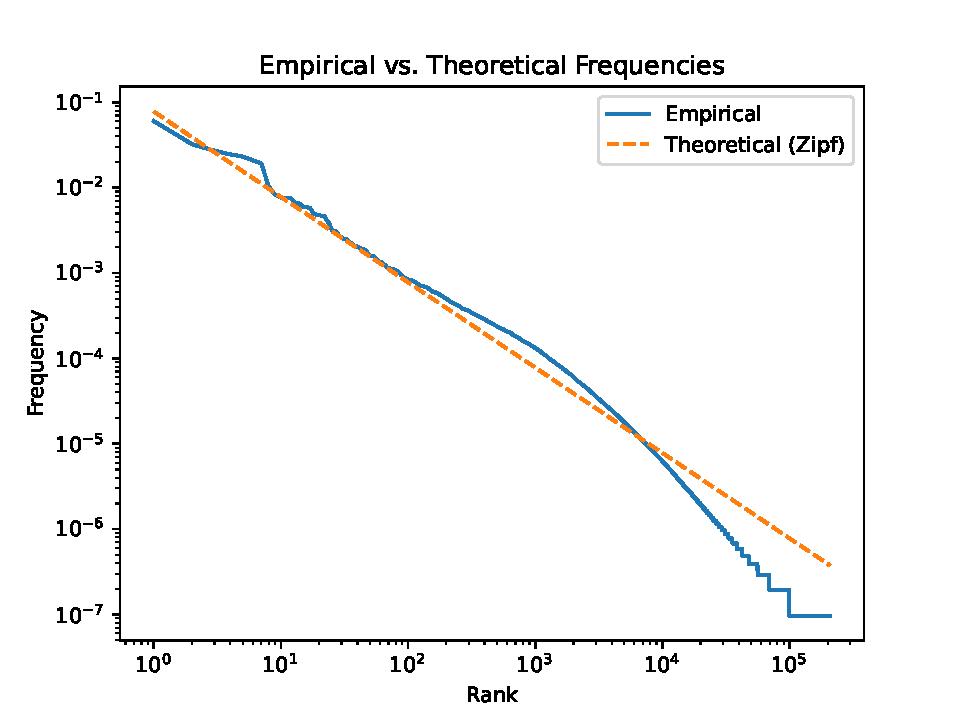
\includegraphics[width=0.45\textwidth]{Task_1_1_fig.pdf}
\caption{Comparison between empirical distribution
and Zipf’s law distribution}
\end{figure}
\subsection*{}
\begin{figure}[ht]
\centering
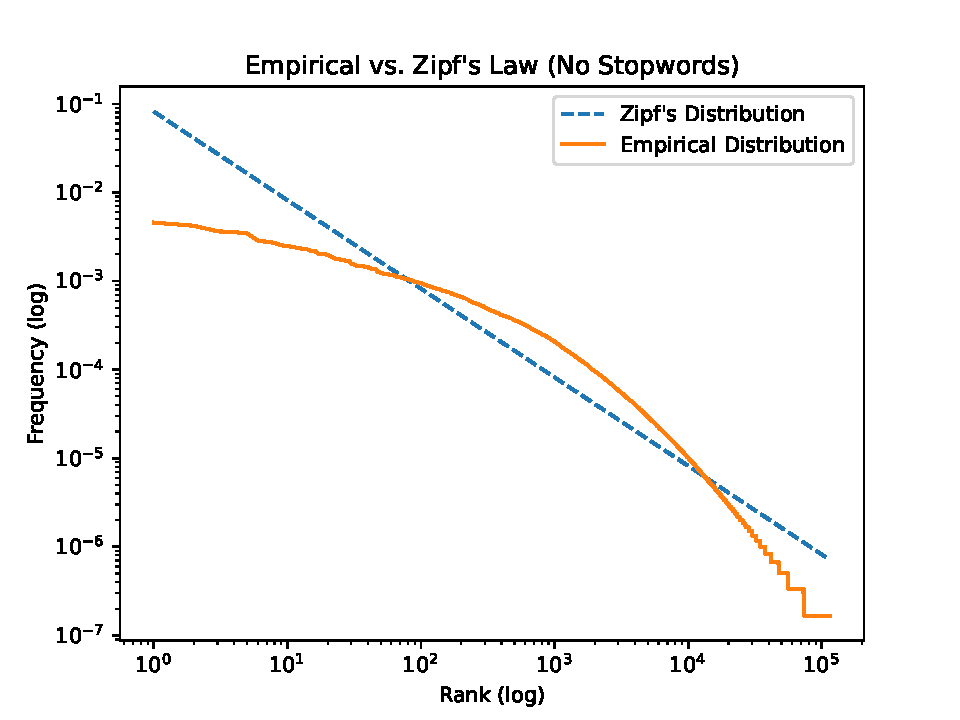
\includegraphics[width=0.45\textwidth]{Task_1_2_fig.pdf}
\caption{Comparison between empirical distribution
and Zipf’s law distribution (log-log scale)}
\end{figure}

\subsection*{}
\begin{figure}[ht]
\centering
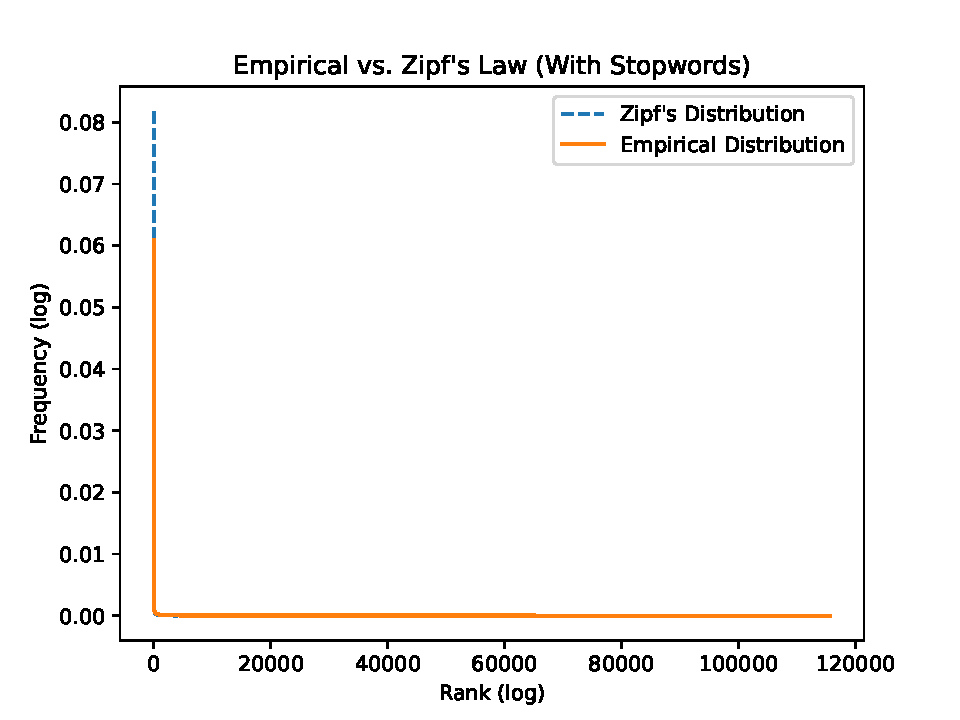
\includegraphics[width=0.45\textwidth]{Task_1_3_fig.pdf}
\caption{Comparison between empirical distribution
and Zipf’s law distribution (log-log scale)}
\end{figure}

\section{Task 2 -- Inverted Index}
To construct an inverted index, the passages in candidate-passages-top1000.tsv are processed using functions developed in Task 1. This preprocessing step involves removing stop words and applying stemming to each token. The function’s output is a two-dimensional list, where each sublist contains tokens extracted from a unique passage. A dictionary is created in the format \{pid: tokens found in the passage\}, mapping passage IDs to their respective tokenised contents.
Next, the inverted index is built. The function iterates through all tokens in the dataset, computing their frequency within each passage. The resulting dictionary format is \{token: \{pid: frequency\}\}, where each token acts as a key, mapping to another dictionary that stores the passage ID (pid) and the corresponding frequency count.
This structure allows efficient retrieval of token occurrences. Given any word, the inverted index provides information on the passages where it appears and its frequency within each passage.

\section{Task 3 -- Retrieval Models}
This task aims to rank passages for each query using two retrieval models: TF-IDF with cosine similarity and BM25. First, each passage is represented as a TF-IDF vector by combining term frequency \(\mathrm{tf}(t,p)\) with inverse document frequency \(\mathrm{idf}(t)\). Specifically, we compute \(\mathrm{idf}(t) = \log_{10}(1 + \frac{\mathrm{df}(t)}{\mathrm{N_{doc}}})\), where \(\mathrm{N_{doc}}\) is the total number of passages and \(\mathrm{df}(t)\) is the number of passages containing the term \(t\). We then calculate the cosine similarity between each query’s TF-IDF vector and every candidate passage, retaining at most the top 100 passages. The results are stored in \texttt{tfidf.csv} with the format \texttt{qid,pid,score}.

Next, we implement BM25 by assigning scores to each query--passage pair with parameters \(k_1 = 1.2\), \(k_2 = 100\), and \(b = 0.75\). Each term’s partial contribution is derived from its document frequency and within-passage frequency, and we similarly select the top 100 passages per query for output. These BM25 results are saved in \texttt{bm25.csv} using the same CSV structure as TF-IDF. Both outputs must have no headers, with lines formatted as \texttt{qid,pid,score}.

\section{Task 4 -- Query likelihood language models}
Dirichlet smoothing produces better results than others. This is due to additive smoothing, including Laplace and Lidstone, which treats all the unseen query tokens equally and possibly overemphasises their importance. In reality, these tokens have different significances. Dirichlet smoothing tackles this issue by adjusting the smoothing amount based on the background probabilities and document length. Hence, Dirichlet is expected to perform better.

This distinction between Dirichlet and additive smoothing is also observed from the query ``what slows down the flow of blood'' which is tokenised to [‘slow’, ‘flow’, ‘blood’]. When inputting this query to the three language models, each model ranked different passages at the top. Below are the three top-ranked passages returned from other models.

\noindent
\textbf{Dirichlet:} ``what slows down the flow of blood \quad What causes esophageal varices? Esophageal varices occur when normal blood flow to your liver is slowed. Liver disease may create scar tissue in the liver which slows the flow of blood. When the blood to your liver is slowed, it begins to back up, leading to an increase of pressure in the major vein (portal vein) that carries blood to your liver.''

\noindent
\textbf{Laplace:} ``what slows down the flow of blood \quad Blood Flow. Blood flow refers to the movement of blood through the vessels from arteries to the capillaries and then into the veins. Pressure is a measure of the force that the blood exerts against the vessel walls as it moves the blood through the vessels.Like all fluids, blood flows from a high pressure area to a region with lower pressure. Blood flows in the same direction as the decreasing pressure gradient: arteries to capillaries to veins...''

\noindent
\textbf{Lidstone:} ``what slows down the flow of blood \quad An aortic aneurysm can also lead to other problems. Blood flow often slows in the bulging section of an aortic aneurysm, causing clots to form. If a blood clot breaks off from an aortic aneurysm in the chest area, it can travel to the brain and cause a stroke...''

As can be seen, Dirichlet smoothing ranks a passage that contains all query tokens. At the same time, Laplace and Lidstone prioritise a general blood discussion in opposition to what causes slow blood flow. It should be noted that Laplace performs worse than Lidstone due to excessive smoothing and pushing less relevant passages higher. This results from a more extensive (\(\epsilon = 1\)) for Laplace, on the other hand, Lidstone is (\(\epsilon = 0.1\)) resulting in a more irrelevant passage from Laplace.

It should be noted that both Laplace and Lidstone smoothing techniques are forms of additive smoothing designed to ensure that the probabilities of unseen tokens are not zero. Laplace and Lidstone are expected to be highly similar because they share the generic formula shown in equation 3, which \(\epsilon=1\) in Laplace:

\[
P(W \mid D) = \frac{\mathrm{tf}_{(w,D)} + \epsilon}{|D| + \epsilon \, |V|} \quad (\text{Equation 3})
\]

In the Lidstone using the value of \(\epsilon=0.1\) is a reasonable choice for our models. This is because the average document length in our text collections is relatively short and the frequency of key words (excluding stop words) is generally minor. Hence, setting \(\epsilon=0.1\) does not give a high probability to unseen tokens. Lidstone models could benefit from a smaller \(\epsilon\) such as \(\epsilon=0.01\) but this is not guaranteed. This could also be why Lidstone performs better than Laplace in the first example query.

I believe a \(\mu = 5000\) for Dirichlet smoothing is not a good choice for the collections of text used in this coursework. This is because the formula for Dirichlet smoothing is like Equation 4. The average text size is 56.78 words, using the formula \( \frac{N}{N+\mu} = 0\) and \(\frac{\mu}{N+\mu} \approx 1\). Hence, this results in probability predominantly dependent on background probability \(P(W \mid C)\), which is not the desired result. Hence \(\mu=50\) is a better value.

\[
P = \frac{N}{N + \mu} P(W \mid D) \;+\; \frac{\mu}{N + \mu} P(W \mid C) \quad (\text{Equation 4})
\]

\end{document}
